\chapter{Resultados}

Com o Agente treinado, é possível gerar novas sequências seguindo a arquitetura ilustrada no módulo de Geração de Sequências.
Neste caso, o Agente gerou mais de 200 proteínas diferentes a partir de mutações na sequência inicial. Destas, 63 possuem um TMScore superior a 92\%.

{\color{red} Imagem do poster TMScore x Numero de proteinas}



%%% Estrutura | TM-Score | Ganho em relacao a inicial | Diferenca da inicial | Diferença da original 

\begin{table}[htbp]
    \centering
    \begin{tabular}{c|cccc}
        \hline
        \textbf{ID} & \textbf{TM-Score} & \textbf{Ganho de TM-Score} & \textbf{IS - seq. inicial} & \textbf{IS - seq. original} \\
        \hline
         1 & 0.9311 & +0.008 pp & 91\% & 31\% \\
         2 & 0.9334 & +0.01 pp & 84\% & 29\% \\
         3 & 0.9343 & +0.011 pp & 82\% & 29\% \\
         4 & 0.9334 & +0.01 pp & 81\% & 28\% \\
        \hline
    \end{tabular}
    \caption{Generated proteins}
    \label{tab:tabela_exemplo}
\end{table}

\begin{figure}%
    \centering
    \subfloat[\centering Estrutura Alvo ]{{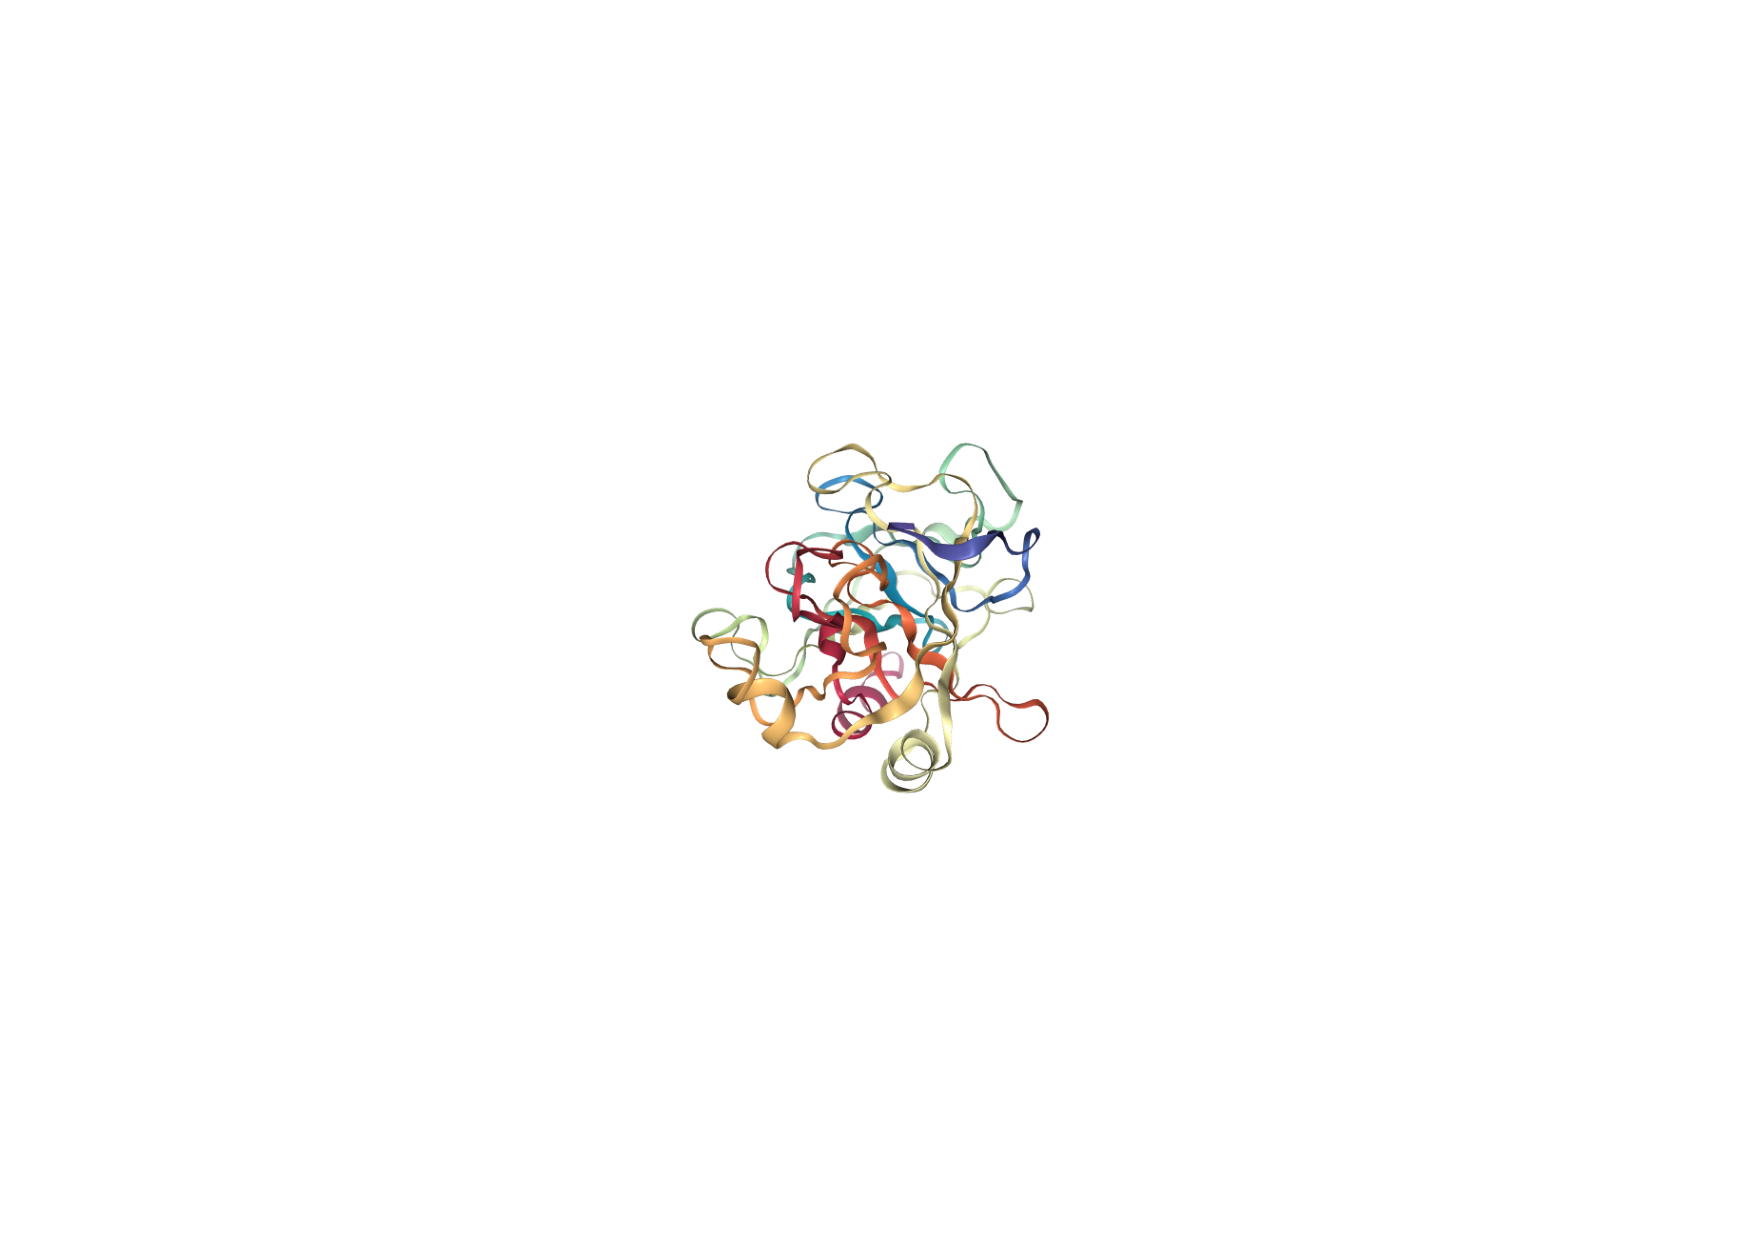
\includegraphics[width=6cm]{figuras/target_structure.pdf} }}%
    \qquad
    \subfloat[\centering Estrutura gerada -  ID 3]{{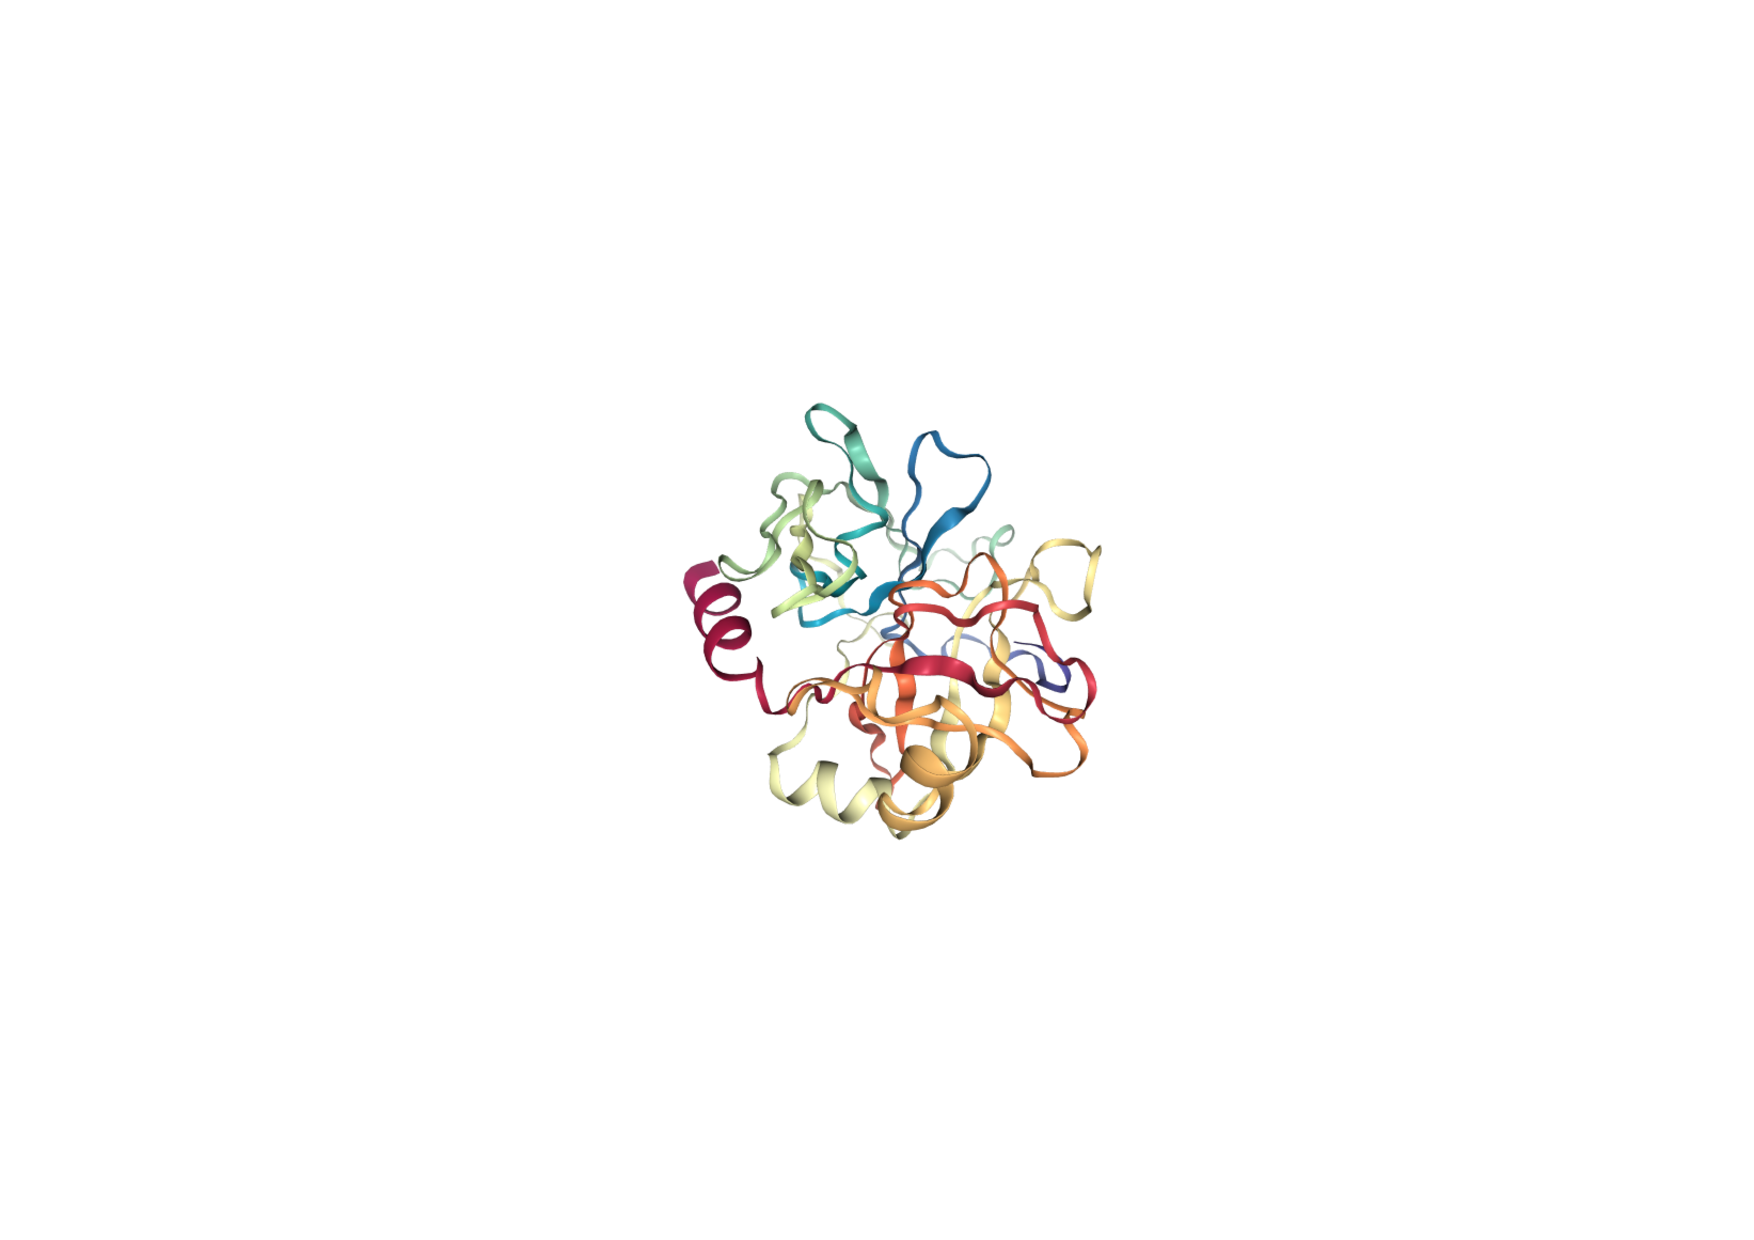
\includegraphics[width=6cm]{figuras/B_v2_tmscore_0.9343_step_41.pdf} }}%
    \caption{Comparação entre estruturas}%
    \label{fig:example}%
\end{figure}

Mesmo reduzindo a IS (Idêntidade de Sequência) em relação a sequência de partida, o Agente foi capaz de produzir sequências que geram um TM-Score ligeiramente superior ao inicial. Isso nos possibilita utilizar o Agente como um gerador de sequências diferentes que se traduzem em estruturas similares.
 